% Beamer slide template prepared by Tom Clark <tom.clark@op.ac.nz>
% Otago Polytechnic
% Dec 2012

\documentclass[10pt]{beamer}
\usetheme{CambridgeUS}
\usepackage{graphicx}
\usepackage{fancyvrb}


\title{Accessing Models with REST and JSON}

\author[IN705]{Databases Three}
\institute[Otago Polytechnic]{
  Otago Polytechnic \\
  Dunedin, New Zealand \\
}
\date{}
\begin{document}

%----------- titlepage ----------------------------------------------%
\begin{frame}[plain]
  \titlepage
\end{frame}



%----------- slide --------------------------------------------------%
\begin{frame}
  \frametitle{Application stack}

   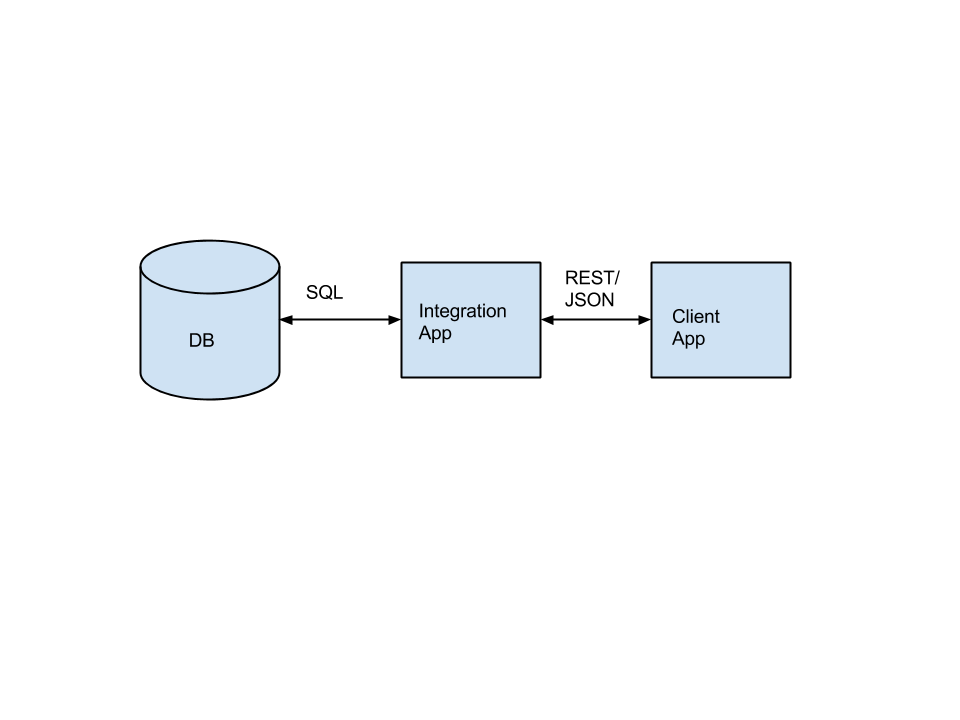
\includegraphics[scale=0.4]{apps.png}


\end{frame}


%----------- slide --------------------------------------------------%
\begin{frame}
  \frametitle{We want to start on the integration app}

 \begin{itemize}
  \item How to we communicate with the DB using SQL?  We use our ORM
        library, \emph{ActiveRecord}.

  \item How to we implement the REST/JSON API?  We use the capabilities of 
        the Rails controller, \emph{ActionController}.
 \end{itemize}

\end{frame}


%----------- slide --------------------------------------------------%
\begin{frame}
  \frametitle{REST}

 \begin{itemize}
  \item Representational State Transfer
  \item Defined by Roy Fielding in 2000\footnote{http://www.ics.uci.edu/\textasciitilde{}fielding/pubs/dissertation/rest\_arch\_style.htm}.
  \item Abstraction of the structure of a certain type of ``well behaved" web applications.
 \end{itemize}

\end{frame}



%----------- slide --------------------------------------------------%
\begin{frame}
  \frametitle{REST}

 Suppose we have a data model that we wish to act upon:
 \begin{itemize}
  \item Create
  \item Read
  \item Update
  \item Delete
 \end{itemize}

\end{frame}


%----------- slide --------------------------------------------------%
\begin{frame}
  \frametitle{REST}

 We can use HTTP to act on the model, mapping HTTP request types, or 
 \emph{verbs}, to CRUD operations.
 \begin{itemize}
  \item Create $\Rightarrow$ POST
  \item Read $\Rightarrow$ GET
  \item Update $\Rightarrow$ PUT
  \item Delete $\Rightarrow$ DELETE
 \end{itemize}

\end{frame}



%----------- slide --------------------------------------------------%
\begin{frame}
  \frametitle{JSON}

 \begin{itemize}
  \item JavaScript Object Notation
  \item Described by Douglas Crockford, ca. 2002
  \item Specified in RFC 7159
 \end{itemize}

\end{frame}



%----------- slide --------------------------------------------------%
\begin{frame}[fragile]
  \frametitle{JSON}

 \begin{verbatim}
  {
    "firstname" : "Tom",
    "lastname" : "Clark",
    "numberOfCats" : 2,
    "contact" : {
      "email" : "tom.clark@op.ac.nz",
      "phone" : "+64 3 470 4356"
    }
  }
 \end{verbatim}

\end{frame}


%----------- slide --------------------------------------------------%
\begin{frame}
  \frametitle{Lab}
  In today's lab we will create a simple application that lets us access a
  simple data model. We will route HTTP requests to controller methods based
  on the HTTP verbs.
  
  \vspace{1\baselineskip}
  We will use JSON to send and receive data about our models.
  
  \vspace{1\baselineskip}
  We will also see how to use \emph{curl} to interact with our application.

\end{frame}



\end{document}
